%
% Copyright (c) 2011-2013, fortiss GmbH.
% Licensed under the Apache License, Version 2.0.
% 
% Use, modification and distribution are subject to the terms specified
% in the accompanying license file LICENSE.txt located at the root directory
% of this software distribution. A copy is available at
% http://chromosome.fortiss.org/.
%
% This file is part of CHROMOSOME.
%
% $Id: example_helloworld.tex 7852 2014-03-14 16:32:01Z geisinger $
%

\section{Example 1: Sensor and Monitor (20 minutes)}
\label{sec:example_sensorMonitor}

We will start by compiling a simple application which is used to collect data from the workstation the application is running on,
such as the free space on a certain partition.
We will then extend the example subsequently in later chapters.

Two steps are required to build an application based on \xme:
first, the build system needs to be generated using CMake
and second the application needs to be compiled using the generated build system.
%In \xme, a different build system tree is generated for every single target node in the network.
%This tutorial will only present how CMake can be used to generate the build system for a Windows-based host system.
%
After the installation of the required prerequisites (see Section~\ref{sec:prereq}), the following steps are required:

\subsection{Configuration on Linux}
\label{sec:example_sensorMonitor:linux}

\begin{enumerate}
	\item Download the source archive of \xme from the website \\
		\url{http://chromosome.fortiss.org/}.
	
	\item Extract the archive to a directory of your choice. Either use a GUI tool or type the following commands in the console:
		
		\texttt{user@host:~> tar -xvzf xme-\xmeVersionNumber{}\xmeVersionSuffix{}-src.tar.gz} \\
		\texttt{user@host:~> cd xme-\xmeVersionNumber{}\xmeVersionSuffix{}-src} \\
		\texttt{user@host:~/xme-\xmeVersionNumber{}\xmeVersionSuffix{}-src> ls} \\
		\verb|AUTHORS.txt  examples  INSTALL.txt  README.txt  THIRDPARTY.txt  VERSION.txt| \\
		\verb|doc          external  LICENSE.txt  tests       tools           xme|
	
		The \texttt{xme-\xmeVersionNumber{}\xmeVersionSuffix{}-src} directory contains \verb|LICENSE.txt|.
		From now on, we will call that directory \verb|<XME_ROOT>|.
	
	\item We will now generate the required build system for building an example node.
		For this purpose, we first create a build directory and then run CMake.
		
		\verb|user@host:XME_ROOT> mkdir -p examples/sensorMonitor/build/sensorNode| \\
		\verb|user@host:XME_ROOT> cd examples/sensorMonitor/build|
		
		From now on, we will call that directory \verb|<BUILD_ROOT>|.
	
	\item The example that we are going to build consists of two nodes.
		Create a subdirectory in \verb|BUILD_ROOT| for the first node:
		
		\verb|user@host:BUILD_ROOT> mkdir sensorNode| \\
		\verb|user@host:BUILD_ROOT> cd sensorNode|
	
	\item Generate the required build system for building the sensor node:
		
		\verb|user@host:BUILD_ROOT/sensorNode> cmake -G "Unix Makefiles" \ | \\
		\verb|                                 ../../src/application/sensorNode|
	
	\item Compile the example:
		
		\verb|user@host:BUILD_ROOT/sensorNode> make|
	
	\item Run the example application:
		
		\verb|user@host:BUILD_ROOT/sensorNode> target/sensorNode|
	
	\item Continue in Section~\ref{sec:example_sensorMonitor:common}.
\end{enumerate}

\subsection{Configuration on Windows}
\label{sec:example_sensorMonitor:windows}

\begin{enumerate}
	\item Download the source archive of \xme from the website \\
		\url{http://chromosome.fortiss.org/}.
	
	\item Extract the archive to a directory of your choice.\footnote{%
		On Windows systems, please ensure that the path name is not extraordinary long, as this could cause issues with the build system (depending on the file system used).}
		After extraction you should see a directory that contains \verb|LICENSE.txt|.
		From now on, we will call that directory \verb|<XME_ROOT>|.
		%The subdirectory \verb|bin| contains binaries shipped with the release.
		%This allows testing of \xme without compiling your own applications.

	\item Use the \emph{start menu} to run \emph{CMake (cmake-gui)} (compare Figure~\ref{fig:cmake_run}).
\begin{figure}[htpb]
	\centering
	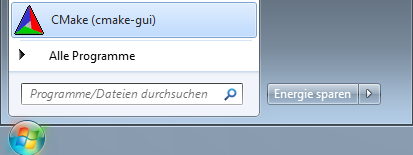
\includegraphics[scale=0.75]{figures/cmake_run.png}
	\caption{\emph{CMake (cmake-gui)} icon in the start menu.}
	\label{fig:cmake_run}
\end{figure}
	\item In the \emph{Where is the source code} field, select the full path to the directory
		\verb|<XME_ROOT>/| \verb|examples/sensorMonitor/src/application/sensorNode| (compare Figure~\ref{fig:cmake_configuration1}).


\begin{figure}[htpb]
	\centering
	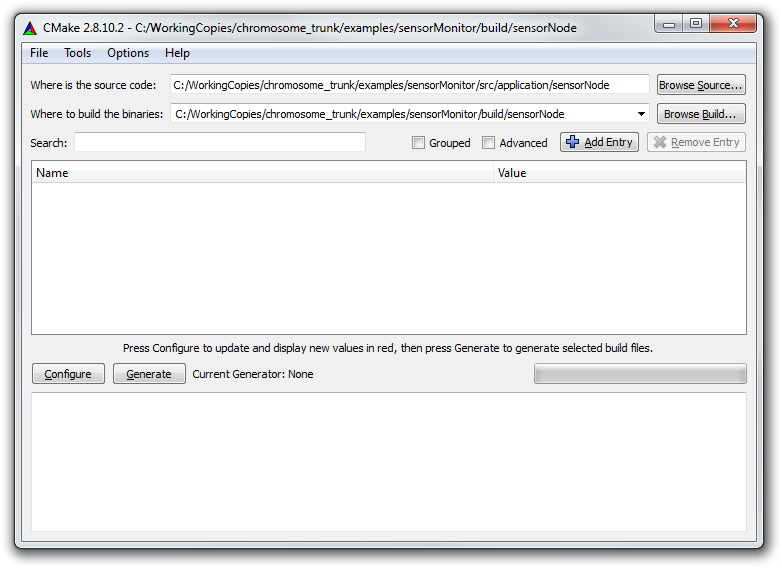
\includegraphics[scale=0.75]{figures/cmake_configuration1.png}
	\caption{Source code and build directory specification.}
	\label{fig:cmake_configuration1}
\end{figure}

	\item In the \emph{Where to build the binaries} field, select the full path to the directory
		\verb|<XME_ROOT>/| \verb|examples/sensorMonitor/build/sensorNode| (note the additional \verb|sensorNode| folder,
		this folder does not yet exist).%\footnote{%
		%This will cause CMake to generate a so-called out-of-source build system, which is recommended.}
	\item Click the \emph{Configure} button.
	\item If asked whether the build directory should be automatically created, say \emph{Yes}.
	\item Choose the \emph{Visual Studio} toolchain that corresponds to your Visual Studio version
		(do \emph{not} use the 64 bit version, even on a 64 bit system) and click \emph{Finish} (compare Figure~\ref{fig:cmake_toolchain}).

\begin{figure}[htpb]
	\centering
	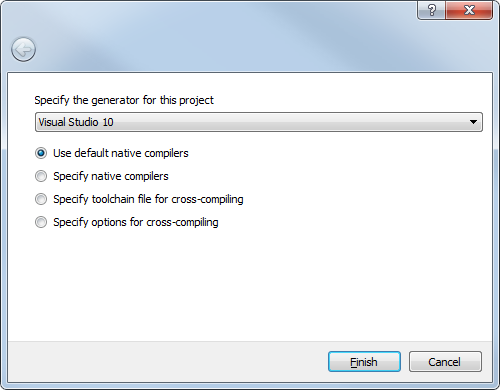
\includegraphics[scale=0.75]{figures/cmake_toolchain.png}
	\caption{Toolchain selection in CMake.}
	\label{fig:cmake_toolchain}
\end{figure}

	\item After CMake has finished its configuration, various configuration variables marked in red should appear in the list
		(compare Figure~\ref{fig:cmake_configuration2}).
	\item Click the \emph{Generate} button.
		This will generate the Visual Studio solution file, called \verb|sensorNode.sln| which you can open in Visual Studio.
		The file will be placed in the following directory: \verb|<XME_ROOT>/examples/sensorMonitor/build/sensorNode| (compare Figure~\ref{fig:build_directory}).

\begin{figure}[h!t]
	\centering
	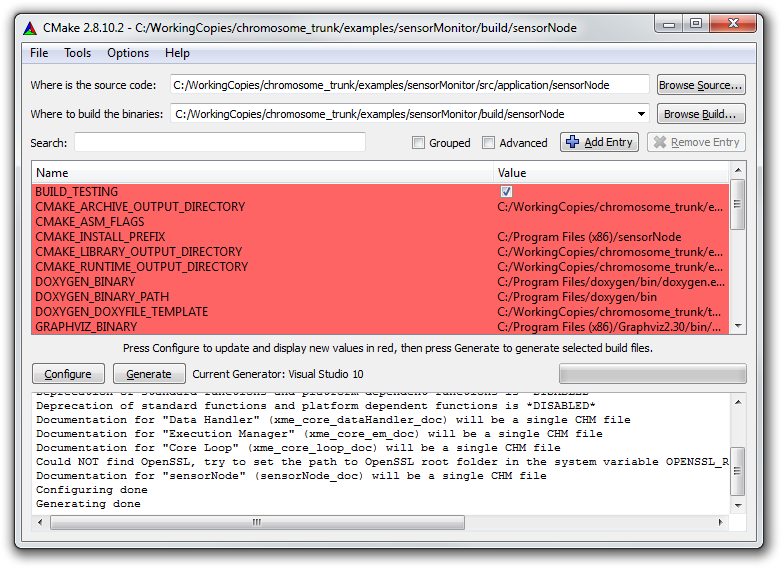
\includegraphics[scale=0.75]{figures/cmake_configuration2.png}
	\caption{Configuration and build system generation in CMake.}
	\label{fig:cmake_configuration2}
\end{figure}

\begin{figure}[htpb]
	\centering
	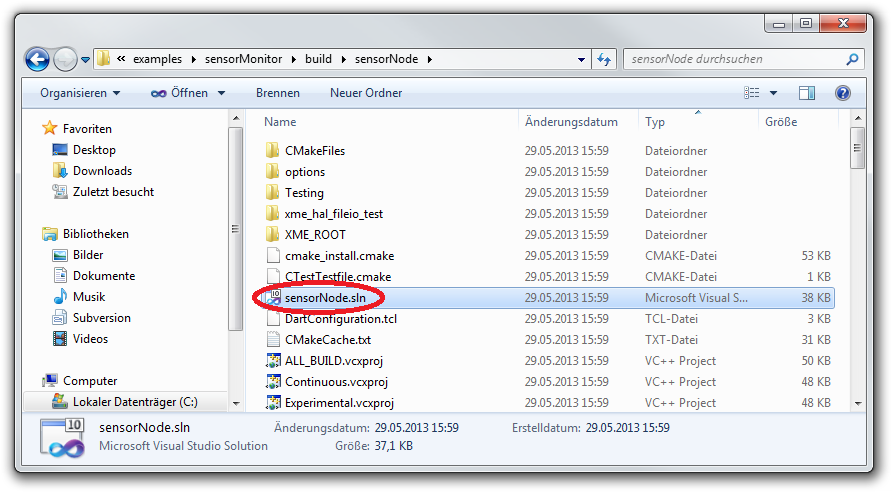
\includegraphics[width=\textwidth]{figures/build_directory_edited.png}
	\caption{Build directory after build system generation, highlighted in red the Visual Studio solution file.}
	\label{fig:build_directory}
\end{figure}

\end{enumerate}

\noindent To compile the exemplified application, the following steps are required:

\begin{enumerate}
	\item Fire up Visual Studio and select \emph{File} $\rightarrow$ \emph{Open} $\rightarrow$ \emph{Project/Solution...}
	\item Navigate to the \verb|<XME_ROOT>/examples/sensorMonitor/build/sensorNode| directory and select the solution file \verb|sensorNode.sln|.
	\item After loading the solution, you will see a project tree in the left-hand pane.
		Right-click on the \verb|sensorNode| project and choose \emph{Set as StartUp Project}
		(compare Figure~\ref{fig:vs_set_as_startup_project}).

\begin{figure}[htpb]
	\centering
	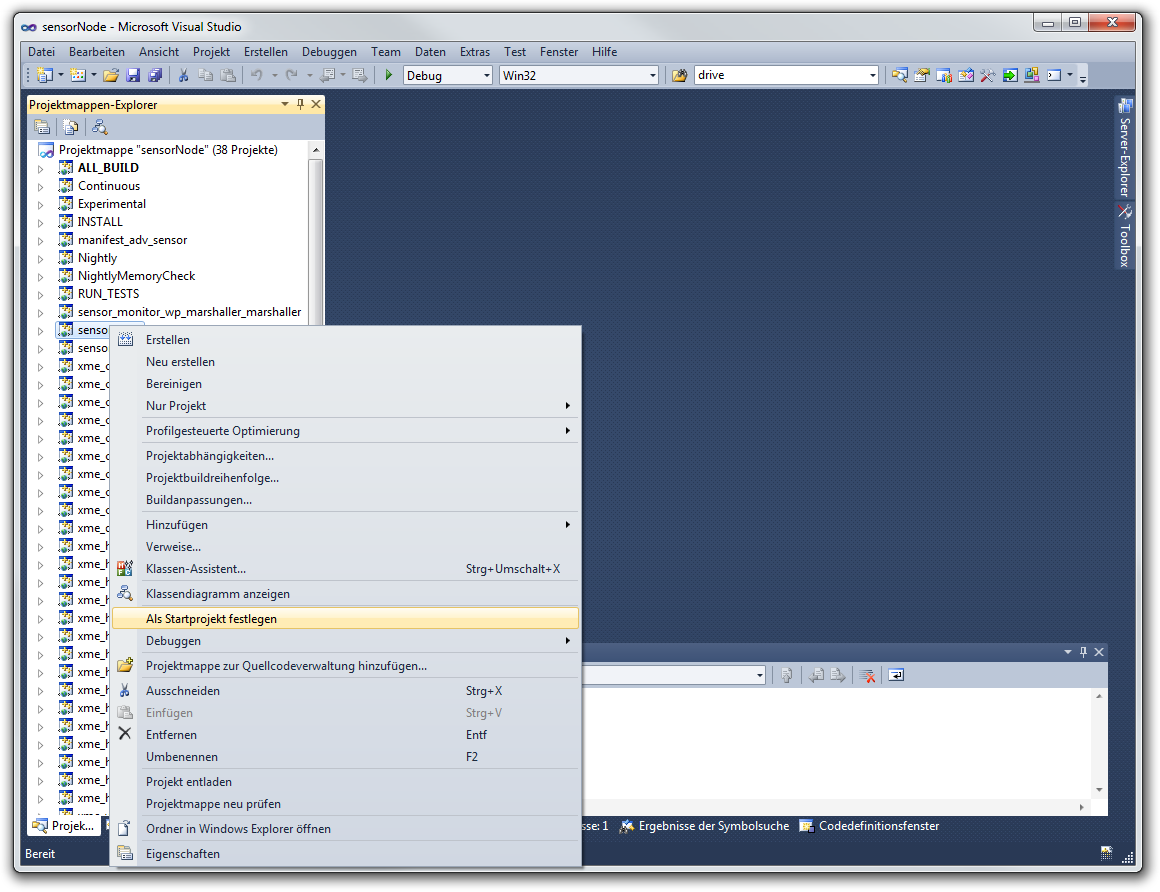
\includegraphics[width=\textwidth]{figures/vs_set_as_startup_project.png}
	\caption{Setting the \texttt{sensorNode} project as \emph{StartUp Project}.}
	\label{fig:vs_set_as_startup_project}
\end{figure}

	\item In the tool bar, select the solution configuration you want to build (usually \texttt{Debug} or \texttt{Release}).
		The \texttt{Debug} build includes debugging information and should be used for development.
		If in doubt, choose \texttt{Debug}.

	\item Hit \emph{F7} to compile the whole solution.

	\item Debug/run the project as usual (e.g., hit \emph{F5} to debug or \emph{Ctrl+F5} to run without debugging).
		If you get prompted whether to rebuild the out-of-date \texttt{ZERO\_CHECK} project (compare Figure~\ref{fig:vs_zero_check}),
		you may select the \emph{Do not show this dialog box again} check box and choose \emph{Yes}.

	\item Continue in Section~\ref{sec:example_sensorMonitor:common}.

\begin{figure}[htpb]
	\centering
	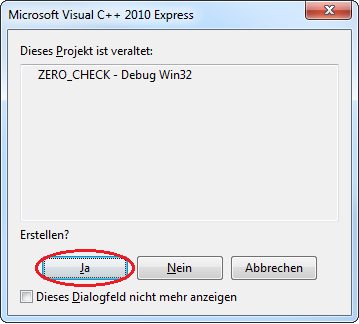
\includegraphics[scale=0.75]{figures/vs_zero_check_edited.png}
	\caption{\texttt{ZERO\_CHECK} project out of date prompt.}
	\label{fig:vs_zero_check}
\end{figure}

\end{enumerate}

\subsection{Notice on Project-global \texttt{CMakeLists.txt} Files}
\label{sec:example_sensorMonitor:projectGlobal}

In \xme, a separate root \texttt{CMakeLists.txt} file is provided for every node.
Thsi is because it could be that each node is to be built for a different target system using a different compiler toolchain.
However, since version 0.8, \xme also support a so-called project-global \texttt{CMakeLists.txt} file per project.
That file is usually located in the root directory of the respective example, say \verb|<XME_ROOT>/examples/sensorMonitor/CMakeLists.txt|.
That file can roughly be undestood as to include all node-specific \texttt{CMakeLists.txt} files.\footnote{%
	With a few exceptions, for example when multiple deployment models exist for a project, see Section~\ref{sec:example_xmt}.%
}
Use the project-global \texttt{CMakeLists.txt} file if all nodes of a project are to be built using the same toolchain for the same target platform.
In this case, it is recommended to name the build directory in the same way as the example itself is named, for example:\\
\verb|<XME_ROOT>/examples/sensorMonitor/build/sensorMonitor|


\subsection{Running the Example Application}
\label{sec:example_sensorMonitor:common}

What you have just compiled is an application that queries simple data from the host it is running on
and makes them accessible to other nodes in the network.
In this case, the collected data is the amount of free space on a certain partition.

When the application starts, you will probably receive a query from the \emph{Windows Firewall}.
\xme is designed to talk to other nodes in the network and hence needs a firewall exception for full functionality.
If you do not want the \xme to talk to other nodes, then simply deny access.\footnote{%
If you want to allow access to the network at a later point in time,
you can change the firewall settings in the \emph{System Control Panel}.}
In this case, communication will be limited to \xme applications on the local computer.
If you want \xme applications to communicate with each other in the local network,
allow access to the \emph{Home or Company Network} as shown in Figure~\ref{fig:firewall_sensorNode}.

\begin{figure}[htpb]
	\centering
	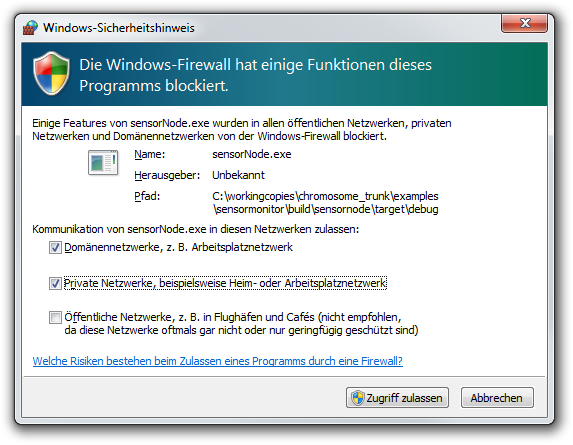
\includegraphics[scale=0.75]{figures/firewall_sensorNode.png}
	\caption{Firewall settings for the \texttt{sensorNode} application.}
	\label{fig:firewall_sensorNode}
\end{figure}

Once the application starts, it presents you with a list of partitions (Linux) or drives (Windows) to choose from.
Select a valid item by entering the respective number.
%
The amount of free space is periodically printed on the console window (compare Figure~\ref{fig:example_sensorNode})
and also transmitted to another \xme node (which is not yet present, see Section~\ref{sec:example_sensorMonitor:monitorNode}).
%
Notice that you can run multiple versions of the sensor node for different partitions/drives on a single host.\footnote{%
	On Windows, when launching the application from within Visual Studio, only one instance can be run at a time.
	In this case, manually navigate to the build directory \texttt{<BUILD\_ROOT>/sensorNode/target} and run the executable from there.
}

The entry point into the executable is in the main source file \verb|<XME_ROOT>/examples/|
\verb|sensorMonitor/src/application/sensorNode/sensorNode.c|,
which also defines the \xme components used in this application.
Notice that this file (and most other files in the example) have been generated from a model.
We will see how this is done in Section~\ref{sec:example_xmt}.
%
%You may now inspect the source code in \verb|sensorNode.c| and the other files related to this example.

\begin{figure}[htpb]
	\centering
	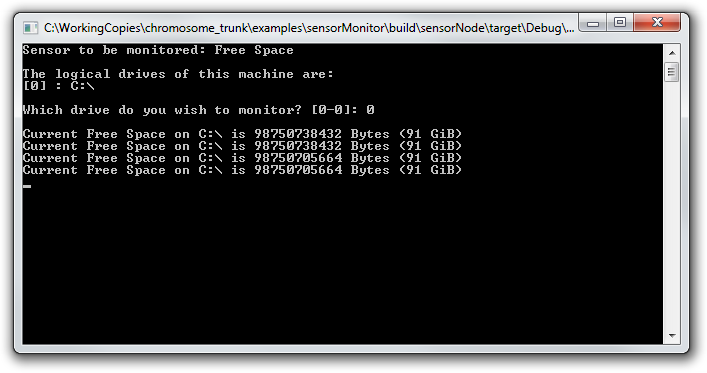
\includegraphics[scale=0.75]{figures/example_sensorNode.png}
	\caption{Sensor node printing free space on drive C: (here on Windows).}
	\label{fig:example_sensorNode}
\end{figure}

\subsection{Compiling and Running the Monitor}
\label{sec:example_sensorMonitor:monitorNode}

Now it's time to compile and run the monitor node that will receive the measurements from the sensor.
Follow the same steps as in Section~\ref{sec:example_sensorMonitor:linux} or Section~\ref{sec:example_sensorMonitor:windows}
(depending on your operating system), but exchange all references to \verb|sensorNode| with \verb|monitorNode|.
On Windows, it is recommended to open a separate Visual Studio instance in order to be able to debug both applications side by side.

When the application starts, you will probably receive another query from the \emph{Windows Firewall}.
Proceed in the same way than for the \verb|sensorNode|.

When launching the \verb|monitorNode| application, you should see the collected data from all sensor nodes on the \emph{current host} being displayed
(compare Figure~\ref{fig:example_monitorNode}).
%
We will shortly come back to remote data transmission in Section~\ref{sec:example_xmt:conclusion}.

\begin{figure}[htpb]
	\centering
	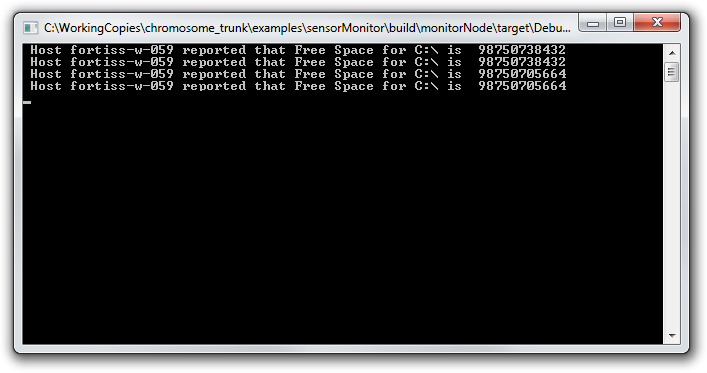
\includegraphics[scale=0.75]{figures/example_monitorNode.png}
	\caption{Monitor node printing free space (here on Windows).}
	\label{fig:example_monitorNode}
\end{figure}
